\documentclass{article}
\usepackage[utf8]{inputenc}
\usepackage[margin=1in]{geometry}
\usepackage{float}
\usepackage{amsmath}
\usepackage{graphicx}
\usepackage{longtable}
\usepackage{tikz}
\usetikzlibrary{patterns}
\usetikzlibrary{plotmarks}

\usepackage[italian]{babel}

\setlength{\parindent}{20pt}
\linespread{1.2}
\title{Misura della caratteristica I-V di un transistor BJT}
\author{Matteo Bonazzi, Massimo D'Alessandro Schmidt}


\begin{document}

\maketitle
\begin{abstract}
    Misura della caratteristica I-V di un transistor BJT in configurazione a emettitore comune, in due valori della corrente di base.\newline
    Dal fit lineare dei dati nella regione attiva, si ottengono i valori $V_{Ea,-100 \,\mu A}=(15.9\pm 0.9) V$ $g_{-100 \,\mu A}=(1.09 \pm 0.06) m\Omega^{-1} $ per la configurazione con $I_b=-100 \mu A$, $V_{Ea,-200 \,\mu A}=(13\pm 1) V $ $g_{-200 \,\mu A}=(2.20 \pm 0.14) m\Omega^{-1}$ per la configurazione con $I_b=-200 \mu A$.\\
    Si stima il guadagno del transistor $\beta=(137\pm38)$.\\
\end{abstract}

\section{Introduzione}
Per la misura è stato utilizato un transistor BJT di tipo pnp, cioè un transistor avente emettitore e colletore fatte di semiconduttore drogato p, e base di semiconduttore drogato n; il transistor è in configurazione a base comune, con base
e collettore collegati a due potenziometri e l'emettitore collegato a terra.\\
Si vogliono misurare la tensione di Early e la resistenza del transistor, da cui si ricava la conduttanza, e si vuole fornire una stima del guadagno in corrente del transistor;
la corrente di Early corrisponde all'intercetta della retta definita dalla caratteristica I-V nella regione attiva, con l'asse delle tensioni.\\
Il circuito è realizzato con due potenziometri regolabili, uno regolante la corrente di base $I_b$ con una resitenza di $100k\Omega$, e uno regolante
la corrente di collettore $I_c$, con resitenza pari a $1k\Omega$, come in figura.
\begin{figure}[H]
    \centering
    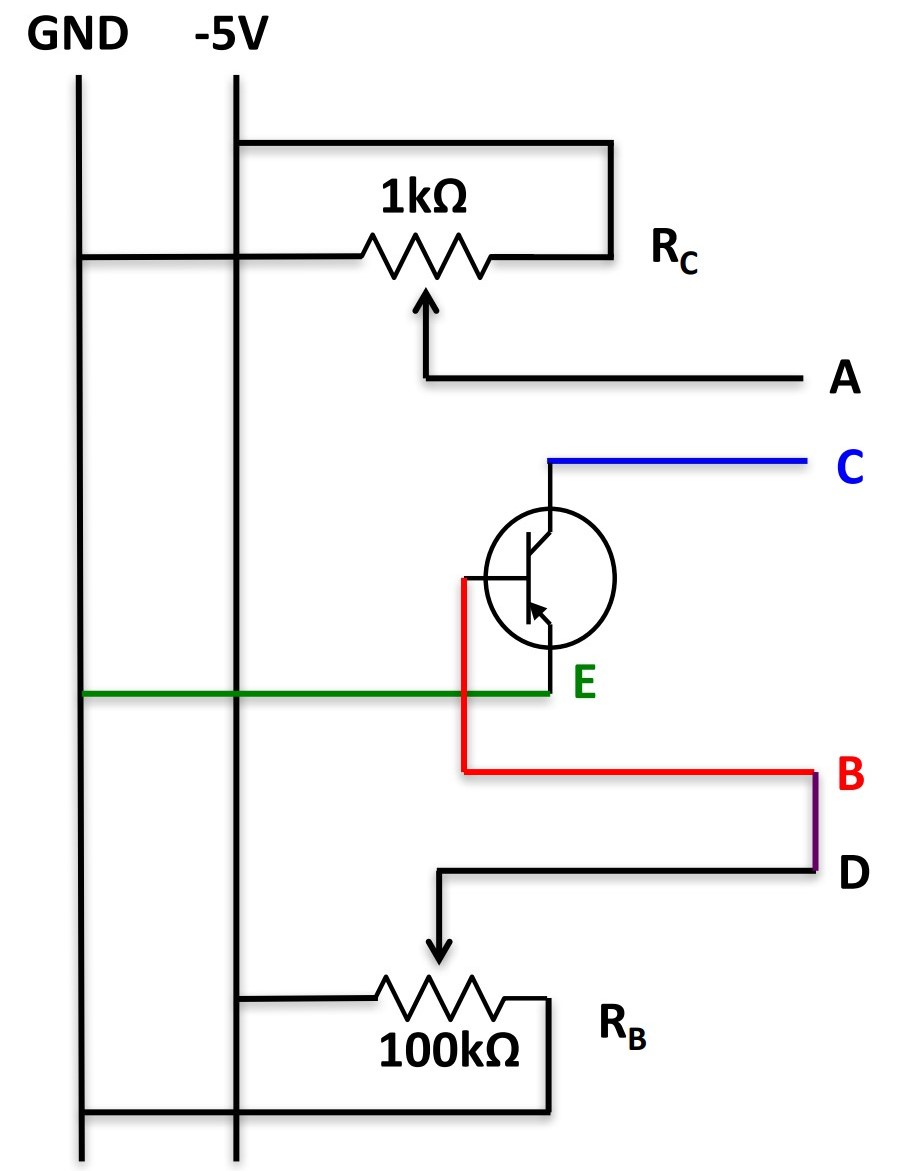
\includegraphics[width=0.3\textwidth]{circuito.jpg}
    \caption{\centering\label{fig:circuito}Foto del circuito realizzato: in alto il potenziometro collegato al collettore, in basso quello collegato alla base; l'emettitore è collegato a terra.}
\end{figure}
Inizialmente si misura la resistenza di base tramite il multimetro, fissandola a $-50 \mu A$, per non bruciare il transistor, e poi si fissa $I_b$ al valore desiderato, misurando la corrente con il multimetro collegato tra i punti B e D.
Prima di misurare la caratteristica è necessario collegare il multimetro ai punti A e C, e l'oscilloscopio al punto C (e al ground); si procede variando la resistenza del potenziometro collegato al collettore e si registrano i valori di voltaggio, dati dall'oscilloscopio, e i valori di corrente, forniti dal multimetro.
È stato scelto di effettuare la maggior parte delle misure nel range $-1 \sim -3 V$, corrispondente alla regione attiva del transistor, per avere una miglior stima del fit; poichè è noto che tutte le grandezze di tensione e corrente misurate sul transistor in questa configurazione sono negative, nel seguito si sceglie di tralasciare il loro segno.
\section{Materiali e strumenti}
Sono stati utilizzati:
\begin{itemize}
    \item Potenzioemtro da $1 k\Omega$
    \item Potenziometro da $100 k\Omega$
    \item Multimetro (Metex M-3650D)
    \item Oscilloscopio (IsoTech ISR622)
    \item Alimentatore a bassa tensione
    \item Transistor pnp 2N3906(BU) al Silicio, in configurazione a emettitore comune
\end{itemize}


\newpage
\section{Analisi dati}

Per $V_{ce}$ nel range $1-4 V$, cioè nella regione attiva del transistor, si opera un fit lineare secondo la funzione:
\begin{equation}
    V_{ce} = a + b I_c\\
\end{equation}
Dove a rappresenta la tensione di Early $V_{Ea}$, e b rappresenta la resistenza del circuito.\\
\begin{figure}[H]
    \begin{center}
        \scalebox{0.7}{\begin{tikzpicture}
\pgfdeclareplotmark{cross} {
\pgfpathmoveto{\pgfpoint{-0.3\pgfplotmarksize}{\pgfplotmarksize}}
\pgfpathlineto{\pgfpoint{+0.3\pgfplotmarksize}{\pgfplotmarksize}}
\pgfpathlineto{\pgfpoint{+0.3\pgfplotmarksize}{0.3\pgfplotmarksize}}
\pgfpathlineto{\pgfpoint{+1\pgfplotmarksize}{0.3\pgfplotmarksize}}
\pgfpathlineto{\pgfpoint{+1\pgfplotmarksize}{-0.3\pgfplotmarksize}}
\pgfpathlineto{\pgfpoint{+0.3\pgfplotmarksize}{-0.3\pgfplotmarksize}}
\pgfpathlineto{\pgfpoint{+0.3\pgfplotmarksize}{-1.\pgfplotmarksize}}
\pgfpathlineto{\pgfpoint{-0.3\pgfplotmarksize}{-1.\pgfplotmarksize}}
\pgfpathlineto{\pgfpoint{-0.3\pgfplotmarksize}{-0.3\pgfplotmarksize}}
\pgfpathlineto{\pgfpoint{-1.\pgfplotmarksize}{-0.3\pgfplotmarksize}}
\pgfpathlineto{\pgfpoint{-1.\pgfplotmarksize}{0.3\pgfplotmarksize}}
\pgfpathlineto{\pgfpoint{-0.3\pgfplotmarksize}{0.3\pgfplotmarksize}}
\pgfpathclose
\pgfusepathqstroke
}
\pgfdeclareplotmark{cross*} {
\pgfpathmoveto{\pgfpoint{-0.3\pgfplotmarksize}{\pgfplotmarksize}}
\pgfpathlineto{\pgfpoint{+0.3\pgfplotmarksize}{\pgfplotmarksize}}
\pgfpathlineto{\pgfpoint{+0.3\pgfplotmarksize}{0.3\pgfplotmarksize}}
\pgfpathlineto{\pgfpoint{+1\pgfplotmarksize}{0.3\pgfplotmarksize}}
\pgfpathlineto{\pgfpoint{+1\pgfplotmarksize}{-0.3\pgfplotmarksize}}
\pgfpathlineto{\pgfpoint{+0.3\pgfplotmarksize}{-0.3\pgfplotmarksize}}
\pgfpathlineto{\pgfpoint{+0.3\pgfplotmarksize}{-1.\pgfplotmarksize}}
\pgfpathlineto{\pgfpoint{-0.3\pgfplotmarksize}{-1.\pgfplotmarksize}}
\pgfpathlineto{\pgfpoint{-0.3\pgfplotmarksize}{-0.3\pgfplotmarksize}}
\pgfpathlineto{\pgfpoint{-1.\pgfplotmarksize}{-0.3\pgfplotmarksize}}
\pgfpathlineto{\pgfpoint{-1.\pgfplotmarksize}{0.3\pgfplotmarksize}}
\pgfpathlineto{\pgfpoint{-0.3\pgfplotmarksize}{0.3\pgfplotmarksize}}
\pgfpathclose
\pgfusepathqfillstroke
}
\pgfdeclareplotmark{newstar} {
\pgfpathmoveto{\pgfqpoint{0pt}{\pgfplotmarksize}}
\pgfpathlineto{\pgfqpointpolar{44}{0.5\pgfplotmarksize}}
\pgfpathlineto{\pgfqpointpolar{18}{\pgfplotmarksize}}
\pgfpathlineto{\pgfqpointpolar{-20}{0.5\pgfplotmarksize}}
\pgfpathlineto{\pgfqpointpolar{-54}{\pgfplotmarksize}}
\pgfpathlineto{\pgfqpointpolar{-90}{0.5\pgfplotmarksize}}
\pgfpathlineto{\pgfqpointpolar{234}{\pgfplotmarksize}}
\pgfpathlineto{\pgfqpointpolar{198}{0.5\pgfplotmarksize}}
\pgfpathlineto{\pgfqpointpolar{162}{\pgfplotmarksize}}
\pgfpathlineto{\pgfqpointpolar{134}{0.5\pgfplotmarksize}}
\pgfpathclose
\pgfusepathqstroke
}
\pgfdeclareplotmark{newstar*} {
\pgfpathmoveto{\pgfqpoint{0pt}{\pgfplotmarksize}}
\pgfpathlineto{\pgfqpointpolar{44}{0.5\pgfplotmarksize}}
\pgfpathlineto{\pgfqpointpolar{18}{\pgfplotmarksize}}
\pgfpathlineto{\pgfqpointpolar{-20}{0.5\pgfplotmarksize}}
\pgfpathlineto{\pgfqpointpolar{-54}{\pgfplotmarksize}}
\pgfpathlineto{\pgfqpointpolar{-90}{0.5\pgfplotmarksize}}
\pgfpathlineto{\pgfqpointpolar{234}{\pgfplotmarksize}}
\pgfpathlineto{\pgfqpointpolar{198}{0.5\pgfplotmarksize}}
\pgfpathlineto{\pgfqpointpolar{162}{\pgfplotmarksize}}
\pgfpathlineto{\pgfqpointpolar{134}{0.5\pgfplotmarksize}}
\pgfpathclose
\pgfusepathqfillstroke
}
\definecolor{c}{rgb}{1,1,1};
\draw [color=c, fill=c] (0,0) rectangle (20,13.639);
\draw [color=c, fill=c] (2,1.3639) rectangle (18,12.2751);
\definecolor{c}{rgb}{0,0,0};
\draw [c,line width=0.9] (2,1.3639) -- (2,12.2751) -- (18,12.2751) -- (18,1.3639) -- (2,1.3639);
\definecolor{c}{rgb}{1,1,1};
\draw [color=c, fill=c] (2,1.3639) rectangle (18,12.2751);
\definecolor{c}{rgb}{0,0,0};
\draw [c,line width=0.9] (2,1.3639) -- (2,12.2751) -- (18,12.2751) -- (18,1.3639) -- (2,1.3639);
\draw [c,line width=0.9] (2,1.3639) -- (18,1.3639);
\draw [c,dash pattern=on 0.80pt off 1.60pt ,line width=0.9] (2.56894,12.2751) -- (2.56894,1.3639);
\draw [c,dash pattern=on 0.80pt off 1.60pt ,line width=0.9] (4.33783,12.2751) -- (4.33783,1.3639);
\draw [c,dash pattern=on 0.80pt off 1.60pt ,line width=0.9] (6.10673,12.2751) -- (6.10673,1.3639);
\draw [c,dash pattern=on 0.80pt off 1.60pt ,line width=0.9] (7.87562,12.2751) -- (7.87562,1.3639);
\draw [c,dash pattern=on 0.80pt off 1.60pt ,line width=0.9] (9.64452,12.2751) -- (9.64452,1.3639);
\draw [c,dash pattern=on 0.80pt off 1.60pt ,line width=0.9] (11.4134,12.2751) -- (11.4134,1.3639);
\draw [c,dash pattern=on 0.80pt off 1.60pt ,line width=0.9] (13.1823,12.2751) -- (13.1823,1.3639);
\draw [c,dash pattern=on 0.80pt off 1.60pt ,line width=0.9] (14.9512,12.2751) -- (14.9512,1.3639);
\draw [c,dash pattern=on 0.80pt off 1.60pt ,line width=0.9] (16.7201,12.2751) -- (16.7201,1.3639);
\draw [c,dash pattern=on 0.80pt off 1.60pt ,line width=0.9] (2.56894,12.2751) -- (2.56894,1.3639);
\draw [c,dash pattern=on 0.80pt off 1.60pt ,line width=0.9] (16.7201,12.2751) -- (16.7201,1.3639);
\draw [c,line width=0.9] (2,1.3639) -- (2,12.2751);
\draw [c,dash pattern=on 0.80pt off 1.60pt ,line width=0.9] (18,2.3913) -- (2,2.3913);
\draw [c,dash pattern=on 0.80pt off 1.60pt ,line width=0.9] (18,3.8386) -- (2,3.8386);
\draw [c,dash pattern=on 0.80pt off 1.60pt ,line width=0.9] (18,5.28591) -- (2,5.28591);
\draw [c,dash pattern=on 0.80pt off 1.60pt ,line width=0.9] (18,6.73322) -- (2,6.73322);
\draw [c,dash pattern=on 0.80pt off 1.60pt ,line width=0.9] (18,8.18052) -- (2,8.18052);
\draw [c,dash pattern=on 0.80pt off 1.60pt ,line width=0.9] (18,9.62783) -- (2,9.62783);
\draw [c,dash pattern=on 0.80pt off 1.60pt ,line width=0.9] (18,11.0751) -- (2,11.0751);
\draw [c,dash pattern=on 0.80pt off 1.60pt ,line width=0.9] (18,2.3913) -- (2,2.3913);
\draw [c,dash pattern=on 0.80pt off 1.60pt ,line width=0.9] (18,11.0751) -- (2,11.0751);
\draw [c,line width=0.9] (2,1.3639) -- (18,1.3639);
\draw [c,line width=0.9] (2.56894,1.69123) -- (2.56894,1.3639);
\draw [c,line width=0.9] (2.92271,1.52756) -- (2.92271,1.3639);
\draw [c,line width=0.9] (3.27649,1.52756) -- (3.27649,1.3639);
\draw [c,line width=0.9] (3.63027,1.52756) -- (3.63027,1.3639);
\draw [c,line width=0.9] (3.98405,1.52756) -- (3.98405,1.3639);
\draw [c,line width=0.9] (4.33783,1.69123) -- (4.33783,1.3639);
\draw [c,line width=0.9] (4.69161,1.52756) -- (4.69161,1.3639);
\draw [c,line width=0.9] (5.04539,1.52756) -- (5.04539,1.3639);
\draw [c,line width=0.9] (5.39917,1.52756) -- (5.39917,1.3639);
\draw [c,line width=0.9] (5.75295,1.52756) -- (5.75295,1.3639);
\draw [c,line width=0.9] (6.10673,1.69123) -- (6.10673,1.3639);
\draw [c,line width=0.9] (6.46051,1.52756) -- (6.46051,1.3639);
\draw [c,line width=0.9] (6.81429,1.52756) -- (6.81429,1.3639);
\draw [c,line width=0.9] (7.16807,1.52756) -- (7.16807,1.3639);
\draw [c,line width=0.9] (7.52184,1.52756) -- (7.52184,1.3639);
\draw [c,line width=0.9] (7.87562,1.69123) -- (7.87562,1.3639);
\draw [c,line width=0.9] (8.2294,1.52756) -- (8.2294,1.3639);
\draw [c,line width=0.9] (8.58318,1.52756) -- (8.58318,1.3639);
\draw [c,line width=0.9] (8.93696,1.52756) -- (8.93696,1.3639);
\draw [c,line width=0.9] (9.29074,1.52756) -- (9.29074,1.3639);
\draw [c,line width=0.9] (9.64452,1.69123) -- (9.64452,1.3639);
\draw [c,line width=0.9] (9.9983,1.52756) -- (9.9983,1.3639);
\draw [c,line width=0.9] (10.3521,1.52756) -- (10.3521,1.3639);
\draw [c,line width=0.9] (10.7059,1.52756) -- (10.7059,1.3639);
\draw [c,line width=0.9] (11.0596,1.52756) -- (11.0596,1.3639);
\draw [c,line width=0.9] (11.4134,1.69123) -- (11.4134,1.3639);
\draw [c,line width=0.9] (11.7672,1.52756) -- (11.7672,1.3639);
\draw [c,line width=0.9] (12.121,1.52756) -- (12.121,1.3639);
\draw [c,line width=0.9] (12.4748,1.52756) -- (12.4748,1.3639);
\draw [c,line width=0.9] (12.8285,1.52756) -- (12.8285,1.3639);
\draw [c,line width=0.9] (13.1823,1.69123) -- (13.1823,1.3639);
\draw [c,line width=0.9] (13.5361,1.52756) -- (13.5361,1.3639);
\draw [c,line width=0.9] (13.8899,1.52756) -- (13.8899,1.3639);
\draw [c,line width=0.9] (14.2436,1.52756) -- (14.2436,1.3639);
\draw [c,line width=0.9] (14.5974,1.52756) -- (14.5974,1.3639);
\draw [c,line width=0.9] (14.9512,1.69123) -- (14.9512,1.3639);
\draw [c,line width=0.9] (15.305,1.52756) -- (15.305,1.3639);
\draw [c,line width=0.9] (15.6588,1.52756) -- (15.6588,1.3639);
\draw [c,line width=0.9] (16.0125,1.52756) -- (16.0125,1.3639);
\draw [c,line width=0.9] (16.3663,1.52756) -- (16.3663,1.3639);
\draw [c,line width=0.9] (16.7201,1.69123) -- (16.7201,1.3639);
\draw [c,line width=0.9] (2.56894,1.69123) -- (2.56894,1.3639);
\draw [c,line width=0.9] (2.21516,1.52756) -- (2.21516,1.3639);
\draw [c,line width=0.9] (16.7201,1.69123) -- (16.7201,1.3639);
\draw [c,line width=0.9] (17.0739,1.52756) -- (17.0739,1.3639);
\draw [c,line width=0.9] (17.4277,1.52756) -- (17.4277,1.3639);
\draw [c,line width=0.9] (17.7814,1.52756) -- (17.7814,1.3639);
\draw [anchor=base] (2.56894,0.913811) node[scale=1.08185, color=c, rotate=0]{0};
\draw [anchor=base] (4.33783,0.913811) node[scale=1.08185, color=c, rotate=0]{500};
\draw [anchor=base] (6.10673,0.913811) node[scale=1.08185, color=c, rotate=0]{1000};
\draw [anchor=base] (7.87562,0.913811) node[scale=1.08185, color=c, rotate=0]{1500};
\draw [anchor=base] (9.64452,0.913811) node[scale=1.08185, color=c, rotate=0]{2000};
\draw [anchor=base] (11.4134,0.913811) node[scale=1.08185, color=c, rotate=0]{2500};
\draw [anchor=base] (13.1823,0.913811) node[scale=1.08185, color=c, rotate=0]{3000};
\draw [anchor=base] (14.9512,0.913811) node[scale=1.08185, color=c, rotate=0]{3500};
\draw [anchor=base] (16.7201,0.913811) node[scale=1.08185, color=c, rotate=0]{4000};
\draw [anchor= east] (18,0.600115) node[scale=1.08185, color=c, rotate=0]{$-V_{ce}  (mV)$};
\draw [c,line width=0.9] (2,1.3639) -- (2,12.2751);
\draw [c,line width=0.9] (2.48,2.3913) -- (2,2.3913);
\draw [c,line width=0.9] (2.24,2.68076) -- (2,2.68076);
\draw [c,line width=0.9] (2.24,2.97022) -- (2,2.97022);
\draw [c,line width=0.9] (2.24,3.25968) -- (2,3.25968);
\draw [c,line width=0.9] (2.24,3.54914) -- (2,3.54914);
\draw [c,line width=0.9] (2.48,3.8386) -- (2,3.8386);
\draw [c,line width=0.9] (2.24,4.12806) -- (2,4.12806);
\draw [c,line width=0.9] (2.24,4.41753) -- (2,4.41753);
\draw [c,line width=0.9] (2.24,4.70699) -- (2,4.70699);
\draw [c,line width=0.9] (2.24,4.99645) -- (2,4.99645);
\draw [c,line width=0.9] (2.48,5.28591) -- (2,5.28591);
\draw [c,line width=0.9] (2.24,5.57537) -- (2,5.57537);
\draw [c,line width=0.9] (2.24,5.86483) -- (2,5.86483);
\draw [c,line width=0.9] (2.24,6.15429) -- (2,6.15429);
\draw [c,line width=0.9] (2.24,6.44376) -- (2,6.44376);
\draw [c,line width=0.9] (2.48,6.73322) -- (2,6.73322);
\draw [c,line width=0.9] (2.24,7.02268) -- (2,7.02268);
\draw [c,line width=0.9] (2.24,7.31214) -- (2,7.31214);
\draw [c,line width=0.9] (2.24,7.6016) -- (2,7.6016);
\draw [c,line width=0.9] (2.24,7.89106) -- (2,7.89106);
\draw [c,line width=0.9] (2.48,8.18052) -- (2,8.18052);
\draw [c,line width=0.9] (2.24,8.46999) -- (2,8.46999);
\draw [c,line width=0.9] (2.24,8.75945) -- (2,8.75945);
\draw [c,line width=0.9] (2.24,9.04891) -- (2,9.04891);
\draw [c,line width=0.9] (2.24,9.33837) -- (2,9.33837);
\draw [c,line width=0.9] (2.48,9.62783) -- (2,9.62783);
\draw [c,line width=0.9] (2.24,9.91729) -- (2,9.91729);
\draw [c,line width=0.9] (2.24,10.2068) -- (2,10.2068);
\draw [c,line width=0.9] (2.24,10.4962) -- (2,10.4962);
\draw [c,line width=0.9] (2.24,10.7857) -- (2,10.7857);
\draw [c,line width=0.9] (2.48,11.0751) -- (2,11.0751);
\draw [c,line width=0.9] (2.48,2.3913) -- (2,2.3913);
\draw [c,line width=0.9] (2.24,2.10183) -- (2,2.10183);
\draw [c,line width=0.9] (2.24,1.81237) -- (2,1.81237);
\draw [c,line width=0.9] (2.24,1.52291) -- (2,1.52291);
\draw [c,line width=0.9] (2.48,11.0751) -- (2,11.0751);
\draw [c,line width=0.9] (2.24,11.3646) -- (2,11.3646);
\draw [c,line width=0.9] (2.24,11.6541) -- (2,11.6541);
\draw [c,line width=0.9] (2.24,11.9435) -- (2,11.9435);
\draw [c,line width=0.9] (2.24,12.233) -- (2,12.233);
\draw [anchor= east] (1.9,2.3913) node[scale=1.08185, color=c, rotate=0]{5};
\draw [anchor= east] (1.9,3.8386) node[scale=1.08185, color=c, rotate=0]{10};
\draw [anchor= east] (1.9,5.28591) node[scale=1.08185, color=c, rotate=0]{15};
\draw [anchor= east] (1.9,6.73322) node[scale=1.08185, color=c, rotate=0]{20};
\draw [anchor= east] (1.9,8.18052) node[scale=1.08185, color=c, rotate=0]{25};
\draw [anchor= east] (1.9,9.62783) node[scale=1.08185, color=c, rotate=0]{30};
\draw [anchor= east] (1.9,11.0751) node[scale=1.08185, color=c, rotate=0]{35};
\draw [anchor= east] (0.784241,12.2751) node[scale=1.08185, color=c, rotate=90]{$-I_c (mA)$};
\definecolor{c}{rgb}{0,0,1};
\draw [c,line width=0.9] (16.7201,7.2253) -- (16.1675,7.2253);
\draw [c,line width=0.9] (16.1675,7.168) -- (16.1675,7.28261);
\draw [c,line width=0.9] (16.7201,7.2253) -- (17.2727,7.2253);
\draw [c,line width=0.9] (17.2727,7.168) -- (17.2727,7.28261);
\draw [c,line width=0.9] (16.7201,7.2253) -- (16.7201,7.32962);
\draw [c,line width=0.9] (16.6628,7.32962) -- (16.7774,7.32962);
\draw [c,line width=0.9] (16.7201,7.2253) -- (16.7201,7.12098);
\draw [c,line width=0.9] (16.6628,7.12098) -- (16.7774,7.12098);
\draw [c,line width=0.9] (16.0125,7.19636) -- (15.4761,7.19636);
\draw [c,line width=0.9] (15.4761,7.13905) -- (15.4761,7.25366);
\draw [c,line width=0.9] (16.0125,7.19636) -- (16.549,7.19636);
\draw [c,line width=0.9] (16.549,7.13905) -- (16.549,7.25366);
\draw [c,line width=0.9] (16.0125,7.19636) -- (16.0125,7.30033);
\draw [c,line width=0.9] (15.9552,7.30033) -- (16.0699,7.30033);
\draw [c,line width=0.9] (16.0125,7.19636) -- (16.0125,7.09238);
\draw [c,line width=0.9] (15.9552,7.09238) -- (16.0699,7.09238);
\draw [c,line width=0.9] (15.305,7.10952) -- (14.7843,7.10952);
\draw [c,line width=0.9] (14.7843,7.05221) -- (14.7843,7.16682);
\draw [c,line width=0.9] (15.305,7.10952) -- (15.8257,7.10952);
\draw [c,line width=0.9] (15.8257,7.05221) -- (15.8257,7.16682);
\draw [c,line width=0.9] (15.305,7.10952) -- (15.305,7.21245);
\draw [c,line width=0.9] (15.2477,7.21245) -- (15.3623,7.21245);
\draw [c,line width=0.9] (15.305,7.10952) -- (15.305,7.00658);
\draw [c,line width=0.9] (15.2477,7.00658) -- (15.3623,7.00658);
\draw [c,line width=0.9] (14.5974,7.05163) -- (14.0921,7.05163);
\draw [c,line width=0.9] (14.0921,6.99432) -- (14.0921,7.10893);
\draw [c,line width=0.9] (14.5974,7.05163) -- (15.1028,7.05163);
\draw [c,line width=0.9] (15.1028,6.99432) -- (15.1028,7.10893);
\draw [c,line width=0.9] (14.5974,7.05163) -- (14.5974,7.15386);
\draw [c,line width=0.9] (14.5401,7.15386) -- (14.6547,7.15386);
\draw [c,line width=0.9] (14.5974,7.05163) -- (14.5974,6.94939);
\draw [c,line width=0.9] (14.5401,6.94939) -- (14.6547,6.94939);
\draw [c,line width=0.9] (13.8899,7.02268) -- (13.5069,7.02268);
\draw [c,line width=0.9] (13.5069,6.96537) -- (13.5069,7.07999);
\draw [c,line width=0.9] (13.8899,7.02268) -- (14.2728,7.02268);
\draw [c,line width=0.9] (14.2728,6.96537) -- (14.2728,7.07999);
\draw [c,line width=0.9] (13.8899,7.02268) -- (13.8899,7.12492);
\draw [c,line width=0.9] (13.8326,7.12492) -- (13.9472,7.12492);
\draw [c,line width=0.9] (13.8899,7.02268) -- (13.8899,6.92044);
\draw [c,line width=0.9] (13.8326,6.92044) -- (13.9472,6.92044);
\draw [c,line width=0.9] (13.1823,7.02268) -- (12.7063,7.02268);
\draw [c,line width=0.9] (12.7063,6.96537) -- (12.7063,7.07999);
\draw [c,line width=0.9] (13.1823,7.02268) -- (13.6583,7.02268);
\draw [c,line width=0.9] (13.6583,6.96537) -- (13.6583,7.07999);
\draw [c,line width=0.9] (13.1823,7.02268) -- (13.1823,7.12492);
\draw [c,line width=0.9] (13.125,7.12492) -- (13.2396,7.12492);
\draw [c,line width=0.9] (13.1823,7.02268) -- (13.1823,6.92044);
\draw [c,line width=0.9] (13.125,6.92044) -- (13.2396,6.92044);
\draw [c,line width=0.9] (12.8285,6.93584) -- (12.4735,6.93584);
\draw [c,line width=0.9] (12.4735,6.87853) -- (12.4735,6.99315);
\draw [c,line width=0.9] (12.8285,6.93584) -- (13.1835,6.93584);
\draw [c,line width=0.9] (13.1835,6.87853) -- (13.1835,6.99315);
\draw [c,line width=0.9] (12.8285,6.93584) -- (12.8285,7.03669);
\draw [c,line width=0.9] (12.7712,7.03669) -- (12.8858,7.03669);
\draw [c,line width=0.9] (12.8285,6.93584) -- (12.8285,6.83499);
\draw [c,line width=0.9] (12.7712,6.83499) -- (12.8858,6.83499);
\draw [c,line width=0.9] (12.121,6.849) -- (11.7842,6.849);
\draw [c,line width=0.9] (11.7842,6.7917) -- (11.7842,6.90631);
\draw [c,line width=0.9] (12.121,6.849) -- (12.4577,6.849);
\draw [c,line width=0.9] (12.4577,6.7917) -- (12.4577,6.90631);
\draw [c,line width=0.9] (12.121,6.849) -- (12.121,6.94881);
\draw [c,line width=0.9] (12.0637,6.94881) -- (12.1783,6.94881);
\draw [c,line width=0.9] (12.121,6.849) -- (12.121,6.7492);
\draw [c,line width=0.9] (12.0637,6.7492) -- (12.1783,6.7492);
\draw [c,line width=0.9] (11.4134,6.849) -- (11.0945,6.849);
\draw [c,line width=0.9] (11.0945,6.7917) -- (11.0945,6.90631);
\draw [c,line width=0.9] (11.4134,6.849) -- (11.7323,6.849);
\draw [c,line width=0.9] (11.7323,6.7917) -- (11.7323,6.90631);
\draw [c,line width=0.9] (11.4134,6.849) -- (11.4134,6.94881);
\draw [c,line width=0.9] (11.3561,6.94881) -- (11.4707,6.94881);
\draw [c,line width=0.9] (11.4134,6.849) -- (11.4134,6.7492);
\draw [c,line width=0.9] (11.3561,6.7492) -- (11.4707,6.7492);
\draw [c,line width=0.9] (11.0596,6.79111) -- (10.7495,6.79111);
\draw [c,line width=0.9] (10.7495,6.7338) -- (10.7495,6.84842);
\draw [c,line width=0.9] (11.0596,6.79111) -- (11.3698,6.79111);
\draw [c,line width=0.9] (11.3698,6.7338) -- (11.3698,6.84842);
\draw [c,line width=0.9] (11.0596,6.79111) -- (11.0596,6.89022);
\draw [c,line width=0.9] (11.0023,6.89022) -- (11.1169,6.89022);
\draw [c,line width=0.9] (11.0596,6.79111) -- (11.0596,6.692);
\draw [c,line width=0.9] (11.0023,6.692) -- (11.1169,6.692);
\draw [c,line width=0.9] (10.3521,6.72164) -- (10.0591,6.72164);
\draw [c,line width=0.9] (10.0591,6.66433) -- (10.0591,6.77895);
\draw [c,line width=0.9] (10.3521,6.72164) -- (10.645,6.72164);
\draw [c,line width=0.9] (10.645,6.66433) -- (10.645,6.77895);
\draw [c,line width=0.9] (10.3521,6.72164) -- (10.3521,6.75342);
\draw [c,line width=0.9] (10.2948,6.75342) -- (10.4094,6.75342);
\draw [c,line width=0.9] (10.3521,6.72164) -- (10.3521,6.68986);
\draw [c,line width=0.9] (10.2948,6.68986) -- (10.4094,6.68986);
\draw [c,line width=0.9] (9.64452,6.6869) -- (9.3682,6.6869);
\draw [c,line width=0.9] (9.3682,6.6296) -- (9.3682,6.74421);
\draw [c,line width=0.9] (9.64452,6.6869) -- (9.92084,6.6869);
\draw [c,line width=0.9] (9.92084,6.6296) -- (9.92084,6.74421);
\draw [c,line width=0.9] (9.64452,6.6869) -- (9.64452,6.71851);
\draw [c,line width=0.9] (9.58721,6.71851) -- (9.70183,6.71851);
\draw [c,line width=0.9] (9.64452,6.6869) -- (9.64452,6.65529);
\draw [c,line width=0.9] (9.58721,6.65529) -- (9.70183,6.65529);
\draw [c,line width=0.9] (9.29074,6.65217) -- (9.02249,6.65217);
\draw [c,line width=0.9] (9.02249,6.59486) -- (9.02249,6.70948);
\draw [c,line width=0.9] (9.29074,6.65217) -- (9.55899,6.65217);
\draw [c,line width=0.9] (9.55899,6.59486) -- (9.55899,6.70948);
\draw [c,line width=0.9] (9.29074,6.65217) -- (9.29074,6.6836);
\draw [c,line width=0.9] (9.23343,6.6836) -- (9.34805,6.6836);
\draw [c,line width=0.9] (9.29074,6.65217) -- (9.29074,6.62073);
\draw [c,line width=0.9] (9.23343,6.62073) -- (9.34805,6.62073);
\draw [c,line width=0.9] (8.58318,6.58559) -- (8.3305,6.58559);
\draw [c,line width=0.9] (8.3305,6.52829) -- (8.3305,6.6429);
\draw [c,line width=0.9] (8.58318,6.58559) -- (8.83586,6.58559);
\draw [c,line width=0.9] (8.83586,6.52829) -- (8.83586,6.6429);
\draw [c,line width=0.9] (8.58318,6.58559) -- (8.58318,6.61669);
\draw [c,line width=0.9] (8.52588,6.61669) -- (8.64049,6.61669);
\draw [c,line width=0.9] (8.58318,6.58559) -- (8.58318,6.55449);
\draw [c,line width=0.9] (8.52588,6.55449) -- (8.64049,6.55449);
\draw [c,line width=0.9] (7.87562,6.51902) -- (7.63764,6.51902);
\draw [c,line width=0.9] (7.63764,6.46171) -- (7.63764,6.57632);
\draw [c,line width=0.9] (7.87562,6.51902) -- (8.11361,6.51902);
\draw [c,line width=0.9] (8.11361,6.46171) -- (8.11361,6.57632);
\draw [c,line width=0.9] (7.87562,6.51902) -- (7.87562,6.54979);
\draw [c,line width=0.9] (7.81832,6.54979) -- (7.93293,6.54979);
\draw [c,line width=0.9] (7.87562,6.51902) -- (7.87562,6.48825);
\draw [c,line width=0.9] (7.81832,6.48825) -- (7.93293,6.48825);
\draw [c,line width=0.9] (7.52184,6.48428) -- (7.29082,6.48428);
\draw [c,line width=0.9] (7.29082,6.42697) -- (7.29082,6.54159);
\draw [c,line width=0.9] (7.52184,6.48428) -- (7.75287,6.48428);
\draw [c,line width=0.9] (7.75287,6.42697) -- (7.75287,6.54159);
\draw [c,line width=0.9] (7.52184,6.48428) -- (7.52184,6.51488);
\draw [c,line width=0.9] (7.46454,6.51488) -- (7.57915,6.51488);
\draw [c,line width=0.9] (7.52184,6.48428) -- (7.52184,6.45368);
\draw [c,line width=0.9] (7.46454,6.45368) -- (7.57915,6.45368);
\draw [c,line width=0.9] (6.81429,6.38876) -- (6.66858,6.38876);
\draw [c,line width=0.9] (6.66858,6.33145) -- (6.66858,6.44606);
\draw [c,line width=0.9] (6.81429,6.38876) -- (6.95999,6.38876);
\draw [c,line width=0.9] (6.95999,6.33145) -- (6.95999,6.44606);
\draw [c,line width=0.9] (6.81429,6.38876) -- (6.81429,6.41888);
\draw [c,line width=0.9] (6.75698,6.41888) -- (6.87159,6.41888);
\draw [c,line width=0.9] (6.81429,6.38876) -- (6.81429,6.35864);
\draw [c,line width=0.9] (6.75698,6.35864) -- (6.87159,6.35864);
\draw [c,line width=0.9] (6.38975,6.35402) -- (6.25504,6.35402);
\draw [c,line width=0.9] (6.25504,6.29672) -- (6.25504,6.41133);
\draw [c,line width=0.9] (6.38975,6.35402) -- (6.52447,6.35402);
\draw [c,line width=0.9] (6.52447,6.29672) -- (6.52447,6.41133);
\draw [c,line width=0.9] (6.38975,6.35402) -- (6.38975,6.38397);
\draw [c,line width=0.9] (6.33244,6.38397) -- (6.44706,6.38397);
\draw [c,line width=0.9] (6.38975,6.35402) -- (6.38975,6.32408);
\draw [c,line width=0.9] (6.33244,6.32408) -- (6.44706,6.32408);
\draw [c,line width=0.9] (6.10673,6.32218) -- (5.97916,6.32218);
\draw [c,line width=0.9] (5.97916,6.26488) -- (5.97916,6.37949);
\draw [c,line width=0.9] (6.10673,6.32218) -- (6.2343,6.32218);
\draw [c,line width=0.9] (6.2343,6.26488) -- (6.2343,6.37949);
\draw [c,line width=0.9] (6.10673,6.32218) -- (6.10673,6.35197);
\draw [c,line width=0.9] (6.04942,6.35197) -- (6.16403,6.35197);
\draw [c,line width=0.9] (6.10673,6.32218) -- (6.10673,6.2924);
\draw [c,line width=0.9] (6.04942,6.2924) -- (6.16403,6.2924);
\draw [c,line width=0.9] (5.39917,6.27587) -- (5.28863,6.27587);
\draw [c,line width=0.9] (5.28863,6.21856) -- (5.28863,6.33318);
\draw [c,line width=0.9] (5.39917,6.27587) -- (5.50971,6.27587);
\draw [c,line width=0.9] (5.50971,6.21856) -- (5.50971,6.33318);
\draw [c,line width=0.9] (5.39917,6.27587) -- (5.39917,6.30542);
\draw [c,line width=0.9] (5.34186,6.30542) -- (5.45648,6.30542);
\draw [c,line width=0.9] (5.39917,6.27587) -- (5.39917,6.24631);
\draw [c,line width=0.9] (5.34186,6.24631) -- (5.45648,6.24631);
\draw [c,line width=0.9] (5.11615,6.23824) -- (5.01199,6.23824);
\draw [c,line width=0.9] (5.01199,6.18093) -- (5.01199,6.29555);
\draw [c,line width=0.9] (5.11615,6.23824) -- (5.2203,6.23824);
\draw [c,line width=0.9] (5.2203,6.18093) -- (5.2203,6.29555);
\draw [c,line width=0.9] (5.11615,6.23824) -- (5.11615,6.2676);
\draw [c,line width=0.9] (5.05884,6.2676) -- (5.17345,6.2676);
\draw [c,line width=0.9] (5.11615,6.23824) -- (5.11615,6.20887);
\draw [c,line width=0.9] (5.05884,6.20887) -- (5.17345,6.20887);
\draw [c,line width=0.9] (4.33783,6.07903) -- (4.27403,6.07903);
\draw [c,line width=0.9] (4.27403,6.02173) -- (4.27403,6.13634);
\draw [c,line width=0.9] (4.33783,6.07903) -- (4.40163,6.07903);
\draw [c,line width=0.9] (4.40163,6.02173) -- (4.40163,6.13634);
\draw [c,line width=0.9] (4.33783,6.07903) -- (4.33783,6.1076);
\draw [c,line width=0.9] (4.28053,6.1076) -- (4.39514,6.1076);
\draw [c,line width=0.9] (4.33783,6.07903) -- (4.33783,6.05046);
\draw [c,line width=0.9] (4.28053,6.05046) -- (4.39514,6.05046);
\draw [c,line width=0.9] (3.98405,5.89667) -- (3.92876,5.89667);
\draw [c,line width=0.9] (3.92876,5.83937) -- (3.92876,5.95398);
\draw [c,line width=0.9] (3.98405,5.89667) -- (4.03934,5.89667);
\draw [c,line width=0.9] (4.03934,5.83937) -- (4.03934,5.95398);
\draw [c,line width=0.9] (3.98405,5.89667) -- (3.98405,5.92433);
\draw [c,line width=0.9] (3.92675,5.92433) -- (4.04136,5.92433);
\draw [c,line width=0.9] (3.98405,5.89667) -- (3.98405,5.86902);
\draw [c,line width=0.9] (3.92675,5.86902) -- (4.04136,5.86902);
\draw [c,line width=0.9] (3.63027,5.51169) -- (3.59381,5.51169);
\draw [c,line width=0.9] (3.59381,5.45438) -- (3.59381,5.569);
\draw [c,line width=0.9] (3.63027,5.51169) -- (3.66674,5.51169);
\draw [c,line width=0.9] (3.66674,5.45438) -- (3.66674,5.569);
\draw [c,line width=0.9] (3.63027,5.51169) -- (3.63027,5.53742);
\draw [c,line width=0.9] (3.57297,5.53742) -- (3.68758,5.53742);
\draw [c,line width=0.9] (3.63027,5.51169) -- (3.63027,5.48596);
\draw [c,line width=0.9] (3.57297,5.48596) -- (3.68758,5.48596);
\draw [c,line width=0.9] (3.27649,4.55068) -- (3.24881,4.55068);
\draw [c,line width=0.9] (3.24881,4.49337) -- (3.24881,4.60799);
\draw [c,line width=0.9] (3.27649,4.55068) -- (3.30418,4.55068);
\draw [c,line width=0.9] (3.30418,4.49337) -- (3.30418,4.60799);
\draw [c,line width=0.9] (3.27649,4.55068) -- (3.27649,4.57161);
\draw [c,line width=0.9] (3.21919,4.57161) -- (3.3338,4.57161);
\draw [c,line width=0.9] (3.27649,4.55068) -- (3.27649,4.52975);
\draw [c,line width=0.9] (3.21919,4.52975) -- (3.3338,4.52975);
\draw [c,line width=0.9] (2.74583,1.86737) -- (2.72727,1.86737);
\draw [c,line width=0.9] (2.72727,1.81006) -- (2.72727,1.92468);
\draw [c,line width=0.9] (2.74583,1.86737) -- (2.76438,1.86737);
\draw [c,line width=0.9] (2.76438,1.81006) -- (2.76438,1.92468);
\draw [c,line width=0.9] (2.74583,1.86737) -- (2.74583,1.87488);
\draw [c,line width=0.9] (2.68852,1.87488) -- (2.80313,1.87488);
\draw [c,line width=0.9] (2.74583,1.86737) -- (2.74583,1.85986);
\draw [c,line width=0.9] (2.68852,1.85986) -- (2.80313,1.85986);
\draw [c,line width=0.9] (16.7201,7.2253) -- (16.0125,7.19636) -- (15.305,7.10952) -- (14.5974,7.05163) -- (13.8899,7.02268) -- (13.1823,7.02268) -- (12.8285,6.93584) -- (12.121,6.849) -- (11.4134,6.849) -- (11.0596,6.79111) -- (10.3521,6.72164) --
 (9.64452,6.6869) -- (9.29074,6.65217) -- (8.58318,6.58559) -- (7.87562,6.51902) -- (7.52184,6.48428) -- (6.81429,6.38876) -- (6.38975,6.35402) -- (6.10673,6.32218) -- (5.39917,6.27587) -- (5.11615,6.23824) -- (4.33783,6.07903) -- (3.98405,5.89667)
 -- (3.63027,5.51169) -- (3.27649,4.55068) -- (2.74583,1.86737);
\definecolor{c}{rgb}{0,0,0};
\foreach \P in {(16.7201,7.2253), (16.0125,7.19636), (15.305,7.10952), (14.5974,7.05163), (13.8899,7.02268), (13.1823,7.02268), (12.8285,6.93584), (12.121,6.849), (11.4134,6.849), (11.0596,6.79111), (10.3521,6.72164), (9.64452,6.6869),
 (9.29074,6.65217), (8.58318,6.58559), (7.87562,6.51902), (7.52184,6.48428), (6.81429,6.38876), (6.38975,6.35402), (6.10673,6.32218), (5.39917,6.27587), (5.11615,6.23824), (4.33783,6.07903), (3.98405,5.89667), (3.63027,5.51169), (3.27649,4.55068),
 (2.74583,1.86737)}{\draw[mark options={color=c,fill=c},mark size=2.402402pt, line width=0.000000pt, mark=*,mark size=1pt] plot coordinates {\P};}
\definecolor{c}{rgb}{1,0,0};
\draw [c,line width=1.8] (6.15979,6.34734) -- (6.26593,6.35689) -- (6.37206,6.36643) -- (6.4782,6.37597) -- (6.58433,6.38552) -- (6.69046,6.39506) -- (6.7966,6.40461) -- (6.90273,6.41415) -- (7.00886,6.42369) -- (7.115,6.43324) -- (7.22113,6.44278)
 -- (7.32727,6.45233) -- (7.4334,6.46187) -- (7.53953,6.47141) -- (7.64567,6.48096) -- (7.7518,6.4905) -- (7.85793,6.50004) -- (7.96407,6.50959) -- (8.0702,6.51913) -- (8.17634,6.52868) -- (8.28247,6.53822) -- (8.3886,6.54776) -- (8.49474,6.55731) --
 (8.60087,6.56685) -- (8.707,6.5764) -- (8.81314,6.58594) -- (8.91927,6.59548) -- (9.02541,6.60503) -- (9.13154,6.61457) -- (9.23767,6.62411) -- (9.34381,6.63366) -- (9.44994,6.6432) -- (9.55608,6.65275) -- (9.66221,6.66229) -- (9.76834,6.67183) --
 (9.87448,6.68138) -- (9.98061,6.69092) -- (10.0867,6.70047) -- (10.1929,6.71001) -- (10.299,6.71955) -- (10.4051,6.7291) -- (10.5113,6.73864) -- (10.6174,6.74818) -- (10.7235,6.75773) -- (10.8297,6.76727) -- (10.9358,6.77682) -- (11.0419,6.78636) --
 (11.1481,6.7959) -- (11.2542,6.80545) -- (11.3603,6.81499);
\draw [c,line width=1.8] (11.3603,6.81499) -- (11.4665,6.82453) -- (11.5726,6.83408) -- (11.6788,6.84362) -- (11.7849,6.85317) -- (11.891,6.86271) -- (11.9972,6.87225) -- (12.1033,6.8818) -- (12.2094,6.89134) -- (12.3156,6.90089) -- (12.4217,6.91043)
 -- (12.5278,6.91997) -- (12.634,6.92952) -- (12.7401,6.93906) -- (12.8462,6.94861) -- (12.9524,6.95815) -- (13.0585,6.96769) -- (13.1646,6.97724) -- (13.2708,6.98678) -- (13.3769,6.99632) -- (13.483,7.00587) -- (13.5892,7.01541) -- (13.6953,7.02496)
 -- (13.8014,7.0345) -- (13.9076,7.04404) -- (14.0137,7.05359) -- (14.1198,7.06313) -- (14.226,7.07267) -- (14.3321,7.08222) -- (14.4382,7.09176) -- (14.5444,7.10131) -- (14.6505,7.11085) -- (14.7566,7.12039) -- (14.8628,7.12994) -- (14.9689,7.13948)
 -- (15.075,7.14903) -- (15.1812,7.15857) -- (15.2873,7.16811) -- (15.3934,7.17766) -- (15.4996,7.1872) -- (15.6057,7.19674) -- (15.7118,7.20629) -- (15.818,7.21583) -- (15.9241,7.22538) -- (16.0302,7.23492) -- (16.1364,7.24446) -- (16.2425,7.25401)
 -- (16.3486,7.26355) -- (16.4548,7.2731) -- (16.5609,7.28264);
\draw [c,line width=1.8] (16.5609,7.28264) -- (16.667,7.29218);
\definecolor{c}{rgb}{0,0,0};
\draw [c,line width=0.9] (16.7201,11.6251) -- (16.1675,11.6251);
\draw [c,line width=0.9] (16.1675,11.5678) -- (16.1675,11.6824);
\draw [c,line width=0.9] (16.7201,11.6251) -- (17.2727,11.6251);
\draw [c,line width=0.9] (17.2727,11.5678) -- (17.2727,11.6824);
\draw [c,line width=0.9] (16.7201,11.6251) -- (16.7201,11.7791);
\draw [c,line width=0.9] (16.6628,11.7791) -- (16.7774,11.7791);
\draw [c,line width=0.9] (16.7201,11.6251) -- (16.7201,11.4711);
\draw [c,line width=0.9] (16.6628,11.4711) -- (16.7774,11.4711);
\draw [c,line width=0.9] (16.0125,11.5093) -- (15.4761,11.5093);
\draw [c,line width=0.9] (15.4761,11.452) -- (15.4761,11.5666);
\draw [c,line width=0.9] (16.0125,11.5093) -- (16.549,11.5093);
\draw [c,line width=0.9] (16.549,11.452) -- (16.549,11.5666);
\draw [c,line width=0.9] (16.0125,11.5093) -- (16.0125,11.6651);
\draw [c,line width=0.9] (15.9552,11.6651) -- (16.0699,11.6651);
\draw [c,line width=0.9] (16.0125,11.5093) -- (16.0125,11.3536);
\draw [c,line width=0.9] (15.9552,11.3536) -- (16.0699,11.3536);
\draw [c,line width=0.9] (15.305,11.3646) -- (14.7843,11.3646);
\draw [c,line width=0.9] (14.7843,11.3073) -- (14.7843,11.4219);
\draw [c,line width=0.9] (15.305,11.3646) -- (15.8257,11.3646);
\draw [c,line width=0.9] (15.8257,11.3073) -- (15.8257,11.4219);
\draw [c,line width=0.9] (15.305,11.3646) -- (15.305,11.5186);
\draw [c,line width=0.9] (15.2477,11.5186) -- (15.3623,11.5186);
\draw [c,line width=0.9] (15.305,11.3646) -- (15.305,11.2106);
\draw [c,line width=0.9] (15.2477,11.2106) -- (15.3623,11.2106);
\draw [c,line width=0.9] (14.5974,11.2488) -- (14.0921,11.2488);
\draw [c,line width=0.9] (14.0921,11.1915) -- (14.0921,11.3061);
\draw [c,line width=0.9] (14.5974,11.2488) -- (15.1028,11.2488);
\draw [c,line width=0.9] (15.1028,11.1915) -- (15.1028,11.3061);
\draw [c,line width=0.9] (14.5974,11.2488) -- (14.5974,11.4014);
\draw [c,line width=0.9] (14.5401,11.4014) -- (14.6547,11.4014);
\draw [c,line width=0.9] (14.5974,11.2488) -- (14.5974,11.0962);
\draw [c,line width=0.9] (14.5401,11.0962) -- (14.6547,11.0962);
\draw [c,line width=0.9] (13.8899,11.1041) -- (13.3995,11.1041);
\draw [c,line width=0.9] (13.3995,11.0468) -- (13.3995,11.1614);
\draw [c,line width=0.9] (13.8899,11.1041) -- (14.3803,11.1041);
\draw [c,line width=0.9] (14.3803,11.0468) -- (14.3803,11.1614);
\draw [c,line width=0.9] (13.8899,11.1041) -- (13.8899,11.255);
\draw [c,line width=0.9] (13.8326,11.255) -- (13.9472,11.255);
\draw [c,line width=0.9] (13.8899,11.1041) -- (13.8899,10.9532);
\draw [c,line width=0.9] (13.8326,10.9532) -- (13.9472,10.9532);
\draw [c,line width=0.9] (13.1823,10.9883) -- (12.7063,10.9883);
\draw [c,line width=0.9] (12.7063,10.931) -- (12.7063,11.0456);
\draw [c,line width=0.9] (13.1823,10.9883) -- (13.6583,10.9883);
\draw [c,line width=0.9] (13.6583,10.931) -- (13.6583,11.0456);
\draw [c,line width=0.9] (13.1823,10.9883) -- (13.1823,11.1378);
\draw [c,line width=0.9] (13.125,11.1378) -- (13.2396,11.1378);
\draw [c,line width=0.9] (13.1823,10.9883) -- (13.1823,10.8388);
\draw [c,line width=0.9] (13.125,10.8388) -- (13.2396,10.8388);
\draw [c,line width=0.9] (12.8285,10.9594) -- (12.4735,10.9594);
\draw [c,line width=0.9] (12.4735,10.902) -- (12.4735,11.0167);
\draw [c,line width=0.9] (12.8285,10.9594) -- (13.1835,10.9594);
\draw [c,line width=0.9] (13.1835,10.902) -- (13.1835,11.0167);
\draw [c,line width=0.9] (12.8285,10.9594) -- (12.8285,11.1085);
\draw [c,line width=0.9] (12.7712,11.1085) -- (12.8858,11.1085);
\draw [c,line width=0.9] (12.8285,10.9594) -- (12.8285,10.8102);
\draw [c,line width=0.9] (12.7712,10.8102) -- (12.8858,10.8102);
\draw [c,line width=0.9] (12.121,10.8436) -- (11.7842,10.8436);
\draw [c,line width=0.9] (11.7842,10.7863) -- (11.7842,10.9009);
\draw [c,line width=0.9] (12.121,10.8436) -- (12.4577,10.8436);
\draw [c,line width=0.9] (12.4577,10.7863) -- (12.4577,10.9009);
\draw [c,line width=0.9] (12.121,10.8436) -- (12.121,10.9913);
\draw [c,line width=0.9] (12.0637,10.9913) -- (12.1783,10.9913);
\draw [c,line width=0.9] (12.121,10.8436) -- (12.121,10.6958);
\draw [c,line width=0.9] (12.0637,10.6958) -- (12.1783,10.6958);
\draw [c,line width=0.9] (11.4134,10.6699) -- (11.0945,10.6699);
\draw [c,line width=0.9] (11.0945,10.6126) -- (11.0945,10.7272);
\draw [c,line width=0.9] (11.4134,10.6699) -- (11.7323,10.6699);
\draw [c,line width=0.9] (11.7323,10.6126) -- (11.7323,10.7272);
\draw [c,line width=0.9] (11.4134,10.6699) -- (11.4134,10.8155);
\draw [c,line width=0.9] (11.3561,10.8155) -- (11.4707,10.8155);
\draw [c,line width=0.9] (11.4134,10.6699) -- (11.4134,10.5242);
\draw [c,line width=0.9] (11.3561,10.5242) -- (11.4707,10.5242);
\draw [c,line width=0.9] (11.0596,10.6699) -- (10.7495,10.6699);
\draw [c,line width=0.9] (10.7495,10.6126) -- (10.7495,10.7272);
\draw [c,line width=0.9] (11.0596,10.6699) -- (11.3698,10.6699);
\draw [c,line width=0.9] (11.3698,10.6126) -- (11.3698,10.7272);
\draw [c,line width=0.9] (11.0596,10.6699) -- (11.0596,10.8155);
\draw [c,line width=0.9] (11.0023,10.8155) -- (11.1169,10.8155);
\draw [c,line width=0.9] (11.0596,10.6699) -- (11.0596,10.5242);
\draw [c,line width=0.9] (11.0023,10.5242) -- (11.1169,10.5242);
\draw [c,line width=0.9] (10.3521,10.5252) -- (10.0591,10.5252);
\draw [c,line width=0.9] (10.0591,10.4679) -- (10.0591,10.5825);
\draw [c,line width=0.9] (10.3521,10.5252) -- (10.645,10.5252);
\draw [c,line width=0.9] (10.645,10.4679) -- (10.645,10.5825);
\draw [c,line width=0.9] (10.3521,10.5252) -- (10.3521,10.6691);
\draw [c,line width=0.9] (10.2948,10.6691) -- (10.4094,10.6691);
\draw [c,line width=0.9] (10.3521,10.5252) -- (10.3521,10.3812);
\draw [c,line width=0.9] (10.2948,10.3812) -- (10.4094,10.3812);
\draw [c,line width=0.9] (9.64452,10.3515) -- (9.3682,10.3515);
\draw [c,line width=0.9] (9.3682,10.2942) -- (9.3682,10.4088);
\draw [c,line width=0.9] (9.64452,10.3515) -- (9.92084,10.3515);
\draw [c,line width=0.9] (9.92084,10.2942) -- (9.92084,10.4088);
\draw [c,line width=0.9] (9.64452,10.3515) -- (9.64452,10.4933);
\draw [c,line width=0.9] (9.58721,10.4933) -- (9.70183,10.4933);
\draw [c,line width=0.9] (9.64452,10.3515) -- (9.64452,10.2096);
\draw [c,line width=0.9] (9.58721,10.2096) -- (9.70183,10.2096);
\draw [c,line width=0.9] (9.29074,10.3515) -- (9.02249,10.3515);
\draw [c,line width=0.9] (9.02249,10.2942) -- (9.02249,10.4088);
\draw [c,line width=0.9] (9.29074,10.3515) -- (9.55899,10.3515);
\draw [c,line width=0.9] (9.55899,10.2942) -- (9.55899,10.4088);
\draw [c,line width=0.9] (9.29074,10.3515) -- (9.29074,10.4933);
\draw [c,line width=0.9] (9.23343,10.4933) -- (9.34805,10.4933);
\draw [c,line width=0.9] (9.29074,10.3515) -- (9.29074,10.2096);
\draw [c,line width=0.9] (9.23343,10.2096) -- (9.34805,10.2096);
\draw [c,line width=0.9] (8.58318,10.2068) -- (8.3305,10.2068);
\draw [c,line width=0.9] (8.3305,10.1494) -- (8.3305,10.2641);
\draw [c,line width=0.9] (8.58318,10.2068) -- (8.83586,10.2068);
\draw [c,line width=0.9] (8.83586,10.1494) -- (8.83586,10.2641);
\draw [c,line width=0.9] (8.58318,10.2068) -- (8.58318,10.3469);
\draw [c,line width=0.9] (8.52588,10.3469) -- (8.64049,10.3469);
\draw [c,line width=0.9] (8.58318,10.2068) -- (8.58318,10.0667);
\draw [c,line width=0.9] (8.52588,10.0667) -- (8.64049,10.0667);
\draw [c,line width=0.9] (7.87562,10.0331) -- (7.63764,10.0331);
\draw [c,line width=0.9] (7.63764,9.97577) -- (7.63764,10.0904);
\draw [c,line width=0.9] (7.87562,10.0331) -- (8.11361,10.0331);
\draw [c,line width=0.9] (8.11361,9.97577) -- (8.11361,10.0904);
\draw [c,line width=0.9] (7.87562,10.0331) -- (7.87562,10.1711);
\draw [c,line width=0.9] (7.81832,10.1711) -- (7.93293,10.1711);
\draw [c,line width=0.9] (7.87562,10.0331) -- (7.87562,9.89506);
\draw [c,line width=0.9] (7.81832,9.89506) -- (7.93293,9.89506);
\draw [c,line width=0.9] (7.52184,9.97519) -- (7.29082,9.97519);
\draw [c,line width=0.9] (7.29082,9.91788) -- (7.29082,10.0325);
\draw [c,line width=0.9] (7.52184,9.97519) -- (7.75287,9.97519);
\draw [c,line width=0.9] (7.75287,9.91788) -- (7.75287,10.0325);
\draw [c,line width=0.9] (7.52184,9.97519) -- (7.52184,10.1125);
\draw [c,line width=0.9] (7.46454,10.1125) -- (7.57915,10.1125);
\draw [c,line width=0.9] (7.52184,9.97519) -- (7.52184,9.83786);
\draw [c,line width=0.9] (7.46454,9.83786) -- (7.57915,9.83786);
\draw [c,line width=0.9] (6.81429,9.8594) -- (6.66858,9.8594);
\draw [c,line width=0.9] (6.66858,9.80209) -- (6.66858,9.91671);
\draw [c,line width=0.9] (6.81429,9.8594) -- (6.95999,9.8594);
\draw [c,line width=0.9] (6.95999,9.80209) -- (6.95999,9.91671);
\draw [c,line width=0.9] (6.81429,9.8594) -- (6.81429,9.99533);
\draw [c,line width=0.9] (6.75698,9.99533) -- (6.87159,9.99533);
\draw [c,line width=0.9] (6.81429,9.8594) -- (6.81429,9.72347);
\draw [c,line width=0.9] (6.75698,9.72347) -- (6.87159,9.72347);
\draw [c,line width=0.9] (6.53126,9.80151) -- (6.39292,9.80151);
\draw [c,line width=0.9] (6.39292,9.7442) -- (6.39292,9.85882);
\draw [c,line width=0.9] (6.53126,9.80151) -- (6.66961,9.80151);
\draw [c,line width=0.9] (6.66961,9.7442) -- (6.66961,9.85882);
\draw [c,line width=0.9] (6.53126,9.80151) -- (6.53126,9.93674);
\draw [c,line width=0.9] (6.47396,9.93674) -- (6.58857,9.93674);
\draw [c,line width=0.9] (6.53126,9.80151) -- (6.53126,9.66627);
\draw [c,line width=0.9] (6.47396,9.66627) -- (6.58857,9.66627);
\draw [c,line width=0.9] (6.10673,9.68572) -- (5.97916,9.68572);
\draw [c,line width=0.9] (5.97916,9.62842) -- (5.97916,9.74303);
\draw [c,line width=0.9] (6.10673,9.68572) -- (6.2343,9.68572);
\draw [c,line width=0.9] (6.2343,9.62842) -- (6.2343,9.74303);
\draw [c,line width=0.9] (6.10673,9.68572) -- (6.10673,9.81957);
\draw [c,line width=0.9] (6.04942,9.81957) -- (6.16403,9.81957);
\draw [c,line width=0.9] (6.10673,9.68572) -- (6.10673,9.55188);
\draw [c,line width=0.9] (6.04942,9.55188) -- (6.16403,9.55188);
\draw [c,line width=0.9] (5.39917,9.56994) -- (5.28863,9.56994);
\draw [c,line width=0.9] (5.28863,9.51263) -- (5.28863,9.62725);
\draw [c,line width=0.9] (5.39917,9.56994) -- (5.50971,9.56994);
\draw [c,line width=0.9] (5.50971,9.51263) -- (5.50971,9.62725);
\draw [c,line width=0.9] (5.39917,9.56994) -- (5.39917,9.7024);
\draw [c,line width=0.9] (5.34186,9.7024) -- (5.45648,9.7024);
\draw [c,line width=0.9] (5.39917,9.56994) -- (5.39917,9.43748);
\draw [c,line width=0.9] (5.34186,9.43748) -- (5.45648,9.43748);
\draw [c,line width=0.9] (5.11615,9.30942) -- (5.01199,9.30942);
\draw [c,line width=0.9] (5.01199,9.25212) -- (5.01199,9.36673);
\draw [c,line width=0.9] (5.11615,9.30942) -- (5.2203,9.30942);
\draw [c,line width=0.9] (5.2203,9.25212) -- (5.2203,9.36673);
\draw [c,line width=0.9] (5.11615,9.30942) -- (5.11615,9.43876);
\draw [c,line width=0.9] (5.05884,9.43876) -- (5.17345,9.43876);
\draw [c,line width=0.9] (5.11615,9.30942) -- (5.11615,9.18009);
\draw [c,line width=0.9] (5.05884,9.18009) -- (5.17345,9.18009);
\draw [c,line width=0.9] (4.33783,8.61472) -- (4.27403,8.61472);
\draw [c,line width=0.9] (4.27403,8.55741) -- (4.27403,8.67202);
\draw [c,line width=0.9] (4.33783,8.61472) -- (4.40163,8.61472);
\draw [c,line width=0.9] (4.40163,8.55741) -- (4.40163,8.67202);
\draw [c,line width=0.9] (4.33783,8.61472) -- (4.33783,8.73571);
\draw [c,line width=0.9] (4.28053,8.73571) -- (4.39514,8.73571);
\draw [c,line width=0.9] (4.33783,8.61472) -- (4.33783,8.49372);
\draw [c,line width=0.9] (4.28053,8.49372) -- (4.39514,8.49372);
\draw [c,line width=0.9] (3.98405,8.00685) -- (3.92876,8.00685);
\draw [c,line width=0.9] (3.92876,7.94954) -- (3.92876,8.06415);
\draw [c,line width=0.9] (3.98405,8.00685) -- (4.03934,8.00685);
\draw [c,line width=0.9] (4.03934,7.94954) -- (4.03934,8.06415);
\draw [c,line width=0.9] (3.98405,8.00685) -- (3.98405,8.12055);
\draw [c,line width=0.9] (3.92675,8.12055) -- (4.04136,8.12055);
\draw [c,line width=0.9] (3.98405,8.00685) -- (3.98405,7.89315);
\draw [c,line width=0.9] (3.92675,7.89315) -- (4.04136,7.89315);
\draw [c,line width=0.9] (3.63027,7.31214) -- (3.59381,7.31214);
\draw [c,line width=0.9] (3.59381,7.25483) -- (3.59381,7.36945);
\draw [c,line width=0.9] (3.63027,7.31214) -- (3.66674,7.31214);
\draw [c,line width=0.9] (3.66674,7.25483) -- (3.66674,7.36945);
\draw [c,line width=0.9] (3.63027,7.31214) -- (3.63027,7.4175);
\draw [c,line width=0.9] (3.57297,7.4175) -- (3.68758,7.4175);
\draw [c,line width=0.9] (3.63027,7.31214) -- (3.63027,7.20678);
\draw [c,line width=0.9] (3.57297,7.20678) -- (3.68758,7.20678);
\draw [c,line width=0.9] (3.27649,5.88799) -- (3.24881,5.88799);
\draw [c,line width=0.9] (3.24881,5.83068) -- (3.24881,5.9453);
\draw [c,line width=0.9] (3.27649,5.88799) -- (3.30418,5.88799);
\draw [c,line width=0.9] (3.30418,5.83068) -- (3.30418,5.9453);
\draw [c,line width=0.9] (3.27649,5.88799) -- (3.27649,5.9156);
\draw [c,line width=0.9] (3.21919,5.9156) -- (3.3338,5.9156);
\draw [c,line width=0.9] (3.27649,5.88799) -- (3.27649,5.86038);
\draw [c,line width=0.9] (3.21919,5.86038) -- (3.3338,5.86038);
\draw [c,line width=0.9] (2.74583,2.24657) -- (2.72727,2.24657);
\draw [c,line width=0.9] (2.72727,2.18926) -- (2.72727,2.30387);
\draw [c,line width=0.9] (2.74583,2.24657) -- (2.76438,2.24657);
\draw [c,line width=0.9] (2.76438,2.18926) -- (2.76438,2.30387);
\draw [c,line width=0.9] (2.74583,2.24657) -- (2.74583,2.25597);
\draw [c,line width=0.9] (2.68852,2.25597) -- (2.80313,2.25597);
\draw [c,line width=0.9] (2.74583,2.24657) -- (2.74583,2.23716);
\draw [c,line width=0.9] (2.68852,2.23716) -- (2.80313,2.23716);
\draw [c,line width=0.9] (16.7201,11.6251) -- (16.0125,11.5093) -- (15.305,11.3646) -- (14.5974,11.2488) -- (13.8899,11.1041) -- (13.1823,10.9883) -- (12.8285,10.9594) -- (12.121,10.8436) -- (11.4134,10.6699) -- (11.0596,10.6699) -- (10.3521,10.5252)
 -- (9.64452,10.3515) -- (9.29074,10.3515) -- (8.58318,10.2068) -- (7.87562,10.0331) -- (7.52184,9.97519) -- (6.81429,9.8594) -- (6.53126,9.80151) -- (6.10673,9.68572) -- (5.39917,9.56994) -- (5.11615,9.30942) -- (4.33783,8.61472) --
 (3.98405,8.00685) -- (3.63027,7.31214) -- (3.27649,5.88799) -- (2.74583,2.24657);
\foreach \P in {(16.7201,11.6251), (16.0125,11.5093), (15.305,11.3646), (14.5974,11.2488), (13.8899,11.1041), (13.1823,10.9883), (12.8285,10.9594), (12.121,10.8436), (11.4134,10.6699), (11.0596,10.6699), (10.3521,10.5252), (9.64452,10.3515),
 (9.29074,10.3515), (8.58318,10.2068), (7.87562,10.0331), (7.52184,9.97519), (6.81429,9.8594), (6.53126,9.80151), (6.10673,9.68572), (5.39917,9.56994), (5.11615,9.30942), (4.33783,8.61472), (3.98405,8.00685), (3.63027,7.31214), (3.27649,5.88799),
 (2.74583,2.24657)}{\draw[mark options={color=c,fill=c},mark size=2.402402pt, line width=0.000000pt, mark=*,mark size=1pt] plot coordinates {\P};}
\definecolor{c}{rgb}{0,1,0};
\draw [c,line width=1.8] (6.15979,9.73959) -- (6.26593,9.75872) -- (6.37206,9.77785) -- (6.4782,9.79698) -- (6.58433,9.81611) -- (6.69046,9.83525) -- (6.7966,9.85438) -- (6.90273,9.87351) -- (7.00886,9.89264) -- (7.115,9.91177) -- (7.22113,9.9309) --
 (7.32727,9.95003) -- (7.4334,9.96917) -- (7.53953,9.9883) -- (7.64567,10.0074) -- (7.7518,10.0266) -- (7.85793,10.0457) -- (7.96407,10.0648) -- (8.0702,10.084) -- (8.17634,10.1031) -- (8.28247,10.1222) -- (8.3886,10.1413) -- (8.49474,10.1605) --
 (8.60087,10.1796) -- (8.707,10.1987) -- (8.81314,10.2179) -- (8.91927,10.237) -- (9.02541,10.2561) -- (9.13154,10.2753) -- (9.23767,10.2944) -- (9.34381,10.3135) -- (9.44994,10.3327) -- (9.55608,10.3518) -- (9.66221,10.3709) -- (9.76834,10.3901) --
 (9.87448,10.4092) -- (9.98061,10.4283) -- (10.0867,10.4475) -- (10.1929,10.4666) -- (10.299,10.4857) -- (10.4051,10.5048) -- (10.5113,10.524) -- (10.6174,10.5431) -- (10.7235,10.5622) -- (10.8297,10.5814) -- (10.9358,10.6005) -- (11.0419,10.6196) --
 (11.1481,10.6388) -- (11.2542,10.6579) -- (11.3603,10.677);
\draw [c,line width=1.8] (11.3603,10.677) -- (11.4665,10.6962) -- (11.5726,10.7153) -- (11.6788,10.7344) -- (11.7849,10.7536) -- (11.891,10.7727) -- (11.9972,10.7918) -- (12.1033,10.811) -- (12.2094,10.8301) -- (12.3156,10.8492) -- (12.4217,10.8683)
 -- (12.5278,10.8875) -- (12.634,10.9066) -- (12.7401,10.9257) -- (12.8462,10.9449) -- (12.9524,10.964) -- (13.0585,10.9831) -- (13.1646,11.0023) -- (13.2708,11.0214) -- (13.3769,11.0405) -- (13.483,11.0597) -- (13.5892,11.0788) -- (13.6953,11.0979)
 -- (13.8014,11.1171) -- (13.9076,11.1362) -- (14.0137,11.1553) -- (14.1198,11.1744) -- (14.226,11.1936) -- (14.3321,11.2127) -- (14.4382,11.2318) -- (14.5444,11.251) -- (14.6505,11.2701) -- (14.7566,11.2892) -- (14.8628,11.3084) -- (14.9689,11.3275)
 -- (15.075,11.3466) -- (15.1812,11.3658) -- (15.2873,11.3849) -- (15.3934,11.404) -- (15.4996,11.4232) -- (15.6057,11.4423) -- (15.7118,11.4614) -- (15.818,11.4806) -- (15.9241,11.4997) -- (16.0302,11.5188) -- (16.1364,11.5379) -- (16.2425,11.5571)
 -- (16.3486,11.5762) -- (16.4548,11.5953) -- (16.5609,11.6145);
\draw [c,line width=1.8] (16.5609,11.6145) -- (16.667,11.6336);
\definecolor{c}{rgb}{1,1,1};
\draw [color=c, fill=c] (11.404,2.40688) rectangle (17.9943,5.30086);
\definecolor{c}{rgb}{0,0,0};
\draw [c,line width=0.9] (11.404,2.40688) -- (17.9943,2.40688);
\draw [c,line width=0.9] (17.9943,2.40688) -- (17.9943,5.30086);
\draw [c,line width=0.9] (17.9943,5.30086) -- (11.404,5.30086);
\draw [c,line width=0.9] (11.404,5.30086) -- (11.404,2.40688);
\draw [anchor=base] (14.7815,4.88123) node[scale=1.08185, color=c, rotate=0]{Punti sperimentali};
\draw [anchor=base west] (13.0516,4.30244) node[scale=1.08185, color=c, rotate=0]{$I_b = 100 \mu A$};
\definecolor{c}{rgb}{1,1,1};
\draw [c, fill=c] (11.6511,4.23009) -- (12.8044,4.23009) -- (12.8044,4.63524) -- (11.6511,4.63524);
\definecolor{c}{rgb}{0,0,1};
\draw [c,line width=0.9] (11.6511,4.43266) -- (12.8044,4.43266);
\definecolor{c}{rgb}{0,0,0};
\foreach \P in {(12.2278,4.43266)}{\draw[mark options={color=c,fill=c},mark size=2.402402pt, line width=0.000000pt, mark=*,mark size=1pt] plot coordinates {\P};}
\draw [anchor=base west] (13.0516,3.72364) node[scale=1.08185, color=c, rotate=0]{$I_b = 200 \mu A$};
\definecolor{c}{rgb}{1,1,1};
\draw [c, fill=c] (11.6511,3.65129) -- (12.8044,3.65129) -- (12.8044,4.05645) -- (11.6511,4.05645);
\definecolor{c}{rgb}{0,0,0};
\draw [c,line width=0.9] (11.6511,3.85387) -- (12.8044,3.85387);
\foreach \P in {(12.2278,3.85387)}{\draw[mark options={color=c,fill=c},mark size=2.402402pt, line width=0.000000pt, mark=*,mark size=1pt] plot coordinates {\P};}
\draw [anchor=base west] (13.0516,3.14484) node[scale=1.08185, color=c, rotate=0]{Fit lineare a $100 \mu A$};
\definecolor{c}{rgb}{0.95,0.95,0.95};
\draw [c] (11.6511,3.07249) -- (12.8044,3.07249) -- (12.8044,3.47765) -- (11.6511,3.47765);
\definecolor{c}{rgb}{1,0,0};
\draw [c,line width=1.8] (11.6511,3.27507) -- (12.8044,3.27507);
\definecolor{c}{rgb}{0,0,0};
\foreach \P in {(12.2278,3.27507)}{\draw[mark options={color=c,fill=c},mark size=2.402402pt, line width=0.000000pt, mark=*,mark size=1pt] plot coordinates {\P};}
\draw [anchor=base west] (13.0516,2.56605) node[scale=1.08185, color=c, rotate=0]{Fit lineare a $200 \mu A$};
\definecolor{c}{rgb}{0.95,0.95,0.95};
\draw [c] (11.6511,2.4937) -- (12.8044,2.4937) -- (12.8044,2.89885) -- (11.6511,2.89885);
\definecolor{c}{rgb}{0,1,0};
\draw [c,line width=1.8] (11.6511,2.69627) -- (12.8044,2.69627);
\definecolor{c}{rgb}{0,0,0};
\foreach \P in {(12.2278,2.69627)}{\draw[mark options={color=c,fill=c},mark size=2.402402pt, line width=0.000000pt, mark=*,mark size=1pt] plot coordinates {\P};}
\draw (10,13.1957) node[scale=1.40004, color=c, rotate=0]{Caratteristiche I-V};
\end{tikzpicture}
}
        \caption{\centering\label{fig:multigraph}Grafico delle caratterste I-V del transistor, nelle due configurazioni delle correnti di base $I_b$; per maggiore chiarezza grafica, di tutte la quantità è graficato l'opposto}
    \end{center}
\end{figure}
Dal fit si ottengono i seguenti valori:
\begin{equation}
    \begin{aligned}
        V_{Ea,-100 \,\mu A}=(15.9\pm 0.9) \;V  \\
        R_{-100 \,\mu A}=(903 \pm 50) \;\Omega \\
        \\
        V_{Ea,-200 \,\mu A}=(13\pm 1) \;V      \\
        R_{-200 \,\mu A}=(458 \pm 31) \;\Omega \\
    \end{aligned}
\end{equation}
Dalle stime fornite dal fit è possibile ricavare i valori delle conduttanze, che risultano essere:
\begin{equation}
    \begin{aligned}
        g_{-100 \,\mu A}=(1.09 \pm 0.06) \;m\Omega^{-1} \\
        g_{-200 \,\mu A}=(2.20 \pm 0.14) \;m\Omega^{-1} \\
    \end{aligned}
\end{equation}
Definendo il guadagno del trasinstor, a tensione fissata, come:
\begin{equation}
    \beta= \frac{\Delta I_c(V)}{\Delta I_b}
\end{equation}
è possibile calclarne il valore a $V_{ce}=3 \;V$ che risulta pari a
\begin{equation}
    \begin{aligned}
        \beta=(137\pm38)
    \end{aligned}
\end{equation}

\section{Conclusioni}
Il guadagno stimato per il transistor è pari a $\beta=(137\pm38)$, mentre le tensioni di Early e i valori della conduttanza a $I_b=-100 \mu A$sono $V_{Ea,-100 \,\mu A}=(15.9\pm 0.9) \,V$ e $g_{-100 \,\mu A}=(1.09 \pm 0.06) \,m\Omega^{-1} $; a $I_b=-200 \mu A$ si ha $V_{Ea,-200 \,\mu A}=(13\pm 1) \,V $ e $g_{200 \, \mu A}=(2.20 \pm 0.14) \,m\Omega^{-1}$.\\
I valori ottenuti per le tensioni di Early si si discostano dal range tipico di valori (50-100 V) per transistor BJT, effetto probabilmente dovuto alla grande variabilità della tensione di Early in base alla struttura interna e al modello di transistor.


\newpage
\section{Appendice}

\subsection{Dati sperimentali}
Nella configurazione con $I_b=-200\mu A$, si misurano i seguenti valori per $V_{ce}$ e $I_c$:
\begin{longtable}[c]{|l|l|l|l|l|l|l|l|l|}
    \cline{1-4} \cline{6-9}
    $V_{ce}$ (mV) & \begin{tabular}[c]{@{}c@{}}Errore V \\ (mV)\end{tabular} & \begin{tabular}[c]{@{}c@{}}Risoluzione \\ (mV)\end{tabular} & \begin{tabular}[c]{@{}c@{}}Fondo scala \\ (mV/div)\end{tabular} &  & $I_c$ (mA) & \begin{tabular}[c]{@{}c@{}}errore $I_c$  \\ (mA)\end{tabular} & \begin{tabular}[c]{@{}c@{}}Risoluzione \\ (mA)\end{tabular} & \begin{tabular}[c]{@{}c@{}}Fondo scala \\ (mA)\end{tabular} \\ \cline{1-4} \cline{6-9}
    \endfirsthead
    \endhead
    4000          & 160                       & 200                       & 1000                      &  & 36.9       & 0.54                      & 0.1                       & 200                       \\ \cline{1-4} \cline{6-9}
    3800          & 150                       & 200                       & 1000                      &  & 36.5       & 0.54                      & 0.1                       & 200                       \\ \cline{1-4} \cline{6-9}
    3600          & 150                       & 200                       & 1000                      &  & 36         & 0.53                      & 0.1                       & 200                       \\ \cline{1-4} \cline{6-9}
    3400          & 143                       & 200                       & 1000                      &  & 35.6       & 0.53                      & 0.1                       & 200                       \\ \cline{1-4} \cline{6-9}
    3200          & 139                       & 200                       & 1000                      &  & 35.1       & 0.52                      & 0.1                       & 200                       \\ \cline{1-4} \cline{6-9}
    3000          & 135                       & 200                       & 1000                      &  & 34.7       & 0.52                      & 0.1                       & 200                       \\ \cline{1-4} \cline{6-9}
    2900          & 100                       & 200                       & 500                       &  & 34.6       & 0.52                      & 0.1                       & 200                       \\ \cline{1-4} \cline{6-9}
    2700          & 95                        & 200                       & 500                       &  & 34.2       & 0.51                      & 0.1                       & 200                       \\ \cline{1-4} \cline{6-9}
    2500          & 90                        & 100                       & 500                       &  & 33.6       & 0.50                      & 0.1                       & 200                       \\ \cline{1-4} \cline{6-9}
    2400          & 88                        & 100                       & 500                       &  & 33.6       & 0.50                      & 0.1                       & 200                       \\ \cline{1-4} \cline{6-9}
    2200          & 83                        & 100                       & 500                       &  & 33.1       & 0.50                      & 0.1                       & 200                       \\ \cline{1-4} \cline{6-9}
    2000          & 78                        & 100                       & 500                       &  & 32.5       & 0.49                      & 0.1                       & 200                       \\ \cline{1-4} \cline{6-9}
    1900          & 76                        & 100                       & 500                       &  & 32.5       & 0.49                      & 0.1                       & 200                       \\ \cline{1-4} \cline{6-9}
    1700          & 71                        & 100                       & 500                       &  & 32         & 0.48                      & 0.1                       & 200                       \\ \cline{1-4} \cline{6-9}
    1500          & 67                        & 100                       & 500                       &  & 31.4       & 0.48                      & 0.1                       & 200                       \\ \cline{1-4} \cline{6-9}
    1400          & 65                        & 100                       & 500                       &  & 31.2       & 0.47                      & 0.1                       & 200                       \\ \cline{1-4} \cline{6-9}
    1200          & 41                        & 40                        & 200                       &  & 30.8       & 0.47                      & 0.1                       & 200                       \\ \cline{1-4} \cline{6-9}
    1120          & 39                        & 40                        & 200                       &  & 30.6       & 0.47                      & 0.1                       & 200                       \\ \cline{1-4} \cline{6-9}
    1000          & 36                        & 40                        & 200                       &  & 30.2       & 0.46                      & 0.1                       & 200                       \\ \cline{1-4} \cline{6-9}
    800           & 31                        & 40                        & 200                       &  & 29.8       & 0.46                      & 0.1                       & 200                       \\ \cline{1-4} \cline{6-9}
    720           & 29                        & 40                        & 200                       &  & 28.9       & 0.45                      & 0.1                       & 200                       \\ \cline{1-4} \cline{6-9}
    500           & 18                        & 20                        & 100                       &  & 26.5       & 0.42                      & 0.1                       & 200                       \\ \cline{1-4} \cline{6-9}
    400           & 16                        & 20                        & 100                       &  & 24.4       & 0.39                      & 0.1                       & 200                       \\ \cline{1-4} \cline{6-9}
    300           & 10                        & 10                        & 50                        &  & 22         & 0.36                      & 0.1                       & 200                       \\ \cline{1-4} \cline{6-9}
    200           & 7.8                       & 10                        & 50                        &  & 17.08      & 0.095                     & 0.01                      & 20                        \\ \cline{1-4} \cline{6-9}
    50            & 5.2                       & 10                        & 50                        &  & 4.5        & 0.033                    & 0.01                      & 20                        \\ \cline{1-4} \cline{6-9}
    \caption{\label{tab:Tabella1}{Valori di $V_{ce}$ e $I_c$, per $I_b=-200\,\mu A$}}                                                                                                                        \\
\end{longtable}

Nella configurazione con $I_b=-100\mu A$, si misurano i seguenti valori per $V_{ce}$ e $I_c$:
\begin{longtable}[c]{|l|l|l|l|l|l|l|l|l|} 
    \cline{1-4} \cline{6-9}
    $V_{ce}$ (mV) & \begin{tabular}[c]{@{}c@{}}Errore V \\ (mV)\end{tabular} & \begin{tabular}[c]{@{}c@{}}Risoluzione \\ (mV)\end{tabular} & \begin{tabular}[c]{@{}c@{}}Fondo scala \\ (mV/div)\end{tabular} &  & $I_c$ (mA) & \begin{tabular}[c]{@{}c@{}}errore $I_c$  \\ (mA)\end{tabular} & \begin{tabular}[c]{@{}c@{}}Risoluzione \\ (mA)\end{tabular} & \begin{tabular}[c]{@{}c@{}}Fondo scala \\ (mA)\end{tabular} \\ \cline{1-4} \cline{6-9}
    \endfirsthead
    \endhead
    4000          & 156                       & 200                       & 1000                       &  & 21.7       & 0.36                      & 0.1                        & 200                        \\ \cline{1-4} \cline{6-9}
    3800          & 152                       & 200                       & 1000                       &  & 21.6       & 0.39                       & 0.1                        & 200                        \\ \cline{1-4} \cline{6-9}
    3600          & 147                       & 200                       & 1000                       &  & 21.3       & 0.36                       & 0.1                        & 200                        \\ \cline{1-4} \cline{6-9}
    3400          & 143                       & 200                       & 1000                       &  & 21.1       & 0.35                       & 0.1                        & 200                        \\ \cline{1-4} \cline{6-9}
    3200          & 108                       & 200                       & 1000                       &  & 21         & 0.35                       & 0.1                        & 200                        \\ \cline{1-4} \cline{6-9}
    3000          & 135                       & 200                       & 1000                       &  & 21         & 0.35                       & 0.1                        & 200                        \\ \cline{1-4} \cline{6-9}
    2900          & 100                       & 100                       & 500                        &  & 20.7       & 0.35                       & 0.1                        & 200                        \\ \cline{1-4} \cline{6-9}
    2700          & 95                        & 100                       & 500                        &  & 20.4       & 0.34                      & 0.1                        & 200                        \\ \cline{1-4} \cline{6-9}
    2500          & 90                        & 100                       & 500                        &  & 20.4       & 0.34                       & 0.1                        & 200                        \\ \cline{1-4} \cline{6-9}
    2400          & 87                        & 100                       & 500                        &  & 20.2       & 0.34                       & 0.1                        & 200                        \\ \cline{1-4} \cline{6-9}
    2200          & 83                        & 100                       & 500                        &  & 19.96      & 0.11                       & 0.01                       & 20                         \\ \cline{1-4} \cline{6-9}
    2000          & 78                        & 100                       & 500                        &  & 19.84      & 0.11                      & 0.01                       & 20                         \\ \cline{1-4} \cline{6-9}
    1900          & 76                        & 100                       & 500                        &  & 19.72      & 0.11                      & 0.01                       & 20                         \\ \cline{1-4} \cline{6-9}
    1700          & 71                        & 100                       & 500                        &  & 19.49      & 0.11                      & 0.01                       & 20                         \\ \cline{1-4} \cline{6-9}
    1500          & 67                        & 100                       & 500                        &  & 19.26      & 0.11                      & 0.01                       & 20                         \\ \cline{1-4} \cline{6-9}
    1400          & 65                        & 100                       & 500                        &  & 19.14      & 0.11                      & 0.01                       & 20                         \\ \cline{1-4} \cline{6-9}
    1200          & 41                        & 50                        & 200                        &  & 18.81      & 0.10                     & 0.01                       & 20                         \\ \cline{1-4} \cline{6-9}
    1080          & 38                        & 50                        & 200                        &  & 18.69      & 0.10                      & 0.01                       & 20                         \\ \cline{1-4} \cline{6-9}
    1000          & 36                        & 50                        & 200                        &  & 18.58      & 0.10                      & 0.01                       & 20                         \\ \cline{1-4} \cline{6-9}
    800           & 31                        & 50                        & 200                        &  & 18.42      & 0.10                      & 0.01                       & 20                         \\ \cline{1-4} \cline{6-9}
    720           & 29                        & 50                        & 200                        &  & 18.29      & 0.10                      & 0.01                       & 20                         \\ \cline{1-4} \cline{6-9}
    500           & 18                        & 20                        & 100                        &  & 17.74      & 0.099                      & 0.01                       & 20                         \\ \cline{1-4} \cline{6-9}
    400           & 15                        & 20                        & 100                        &  & 17.11      & 0.096                      & 0.01                       & 20                         \\ \cline{1-4} \cline{6-9}
    300           & 10                        & 10                        & 50                         &  & 15.78      & 0.089                      & 0.01                       & 20                         \\ \cline{1-4} \cline{6-9}
    200           & 8                         & 10                        & 50                         &  & 12.46      & 0.072                      & 0.01                       & 20                         \\ \cline{1-4} \cline{6-9}
    50            & 5                         & 10                        & 50                         &  & 3.19       & 0.026                      & 0.01                       & 20                         \\ \cline{1-4} \cline{6-9}
    
    \caption{\label{tab:Tabella2}{Valori di $V_{ce}$ e $I_c$, per $I_b=-100\,\mu A$}}                                                                                                                            \\
\end{longtable}


\subsection{Calcolo degli errori}
Per il calcolo degli errori sulle correnti, si fa riferimento alle informazioni fornite dal costruttore del multimetro:
\begin{figure}[H]
    \centering
    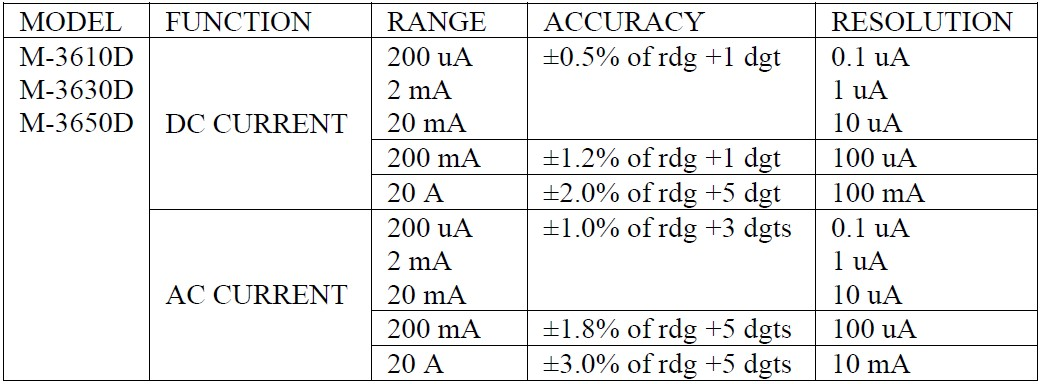
\includegraphics[width=0.7\textwidth]{Errore_multimetro.jpg}
\end{figure}
Per il calcolo degli errori sul multimetro, si utilizza la seguente formula:
\begin{equation}
    \sigma=\sqrt{\sigma_c^2+\sigma_l^2+\sigma_z^2}
\end{equation}
con $\sigma_c^2 = misura*0.03$ errore del costruttore, $\sigma_l^2= \frac{fondo scala}{5}*1/2$ errore sulla lettura (con apprezabilità di mezza tacchetta sull'oscilloscopio) e $\sigma_z^2= \frac{fondo scala}{5}*1/2$ errore sullo zero.
\end{document}